\documentclass[12pt]{report}
\usepackage[utf8]{inputenc}
\usepackage[russian]{babel}
%\usepackage[14pt]{extsizes}
\usepackage{listings}
\usepackage{graphicx}
\usepackage{amsmath,amsfonts,amssymb,amsthm,mathtools} 
\usepackage{pgfplots}
\usepackage{filecontents}
\usepackage{float}
\usepackage{indentfirst}
\usepackage{eucal}
\usepackage{enumitem}
%s\documentclass[openany]{book}
\frenchspacing

\usepackage{indentfirst} % Красная строка

\usetikzlibrary{datavisualization}
\usetikzlibrary{datavisualization.formats.functions}

\usepackage{amsmath}


% Для листинга кода:
\lstset{ %
	language=c,                 % выбор языка для подсветки (здесь это С)
	basicstyle=\small\sffamily, % размер и начертание шрифта для подсветки кода
	numbers=left,               % где поставить нумерацию строк (слева\справа)
	numberstyle=\tiny,           % размер шрифта для номеров строк
	stepnumber=1,                   % размер шага между двумя номерами строк
	numbersep=5pt,                % как далеко отстоят номера строк от подсвечиваемого кода
	showspaces=false,            % показывать или нет пробелы специальными отступами
	showstringspaces=false,      % показывать или нет пробелы в строках
	showtabs=false,             % показывать или нет табуляцию в строках
	frame=single,              % рисовать рамку вокруг кода
	tabsize=2,                 % размер табуляции по умолчанию равен 2 пробелам
	captionpos=t,              % позиция заголовка вверху [t] или внизу [b] 
	breaklines=true,           % автоматически переносить строки (да\нет)
	breakatwhitespace=false, % переносить строки только если есть пробел
	escapeinside={\#*}{*)}   % если нужно добавить комментарии в коде
}


\usepackage[left=2cm,right=2cm, top=2cm,bottom=2cm,bindingoffset=0cm]{geometry}
% Для измененных титулов глав:
\usepackage{titlesec, blindtext, color} % подключаем нужные пакеты
\definecolor{gray75}{gray}{0.75} % определяем цвет
\newcommand{\hsp}{\hspace{20pt}} % длина линии в 20pt
% titleformat определяет стиль
\titleformat{\chapter}[hang]{\Huge\bfseries}{\thechapter\hsp\textcolor{gray75}{|}\hsp}{0pt}{\Huge\bfseries}


% plot
\usepackage{pgfplots}
\usepackage{filecontents}
\usetikzlibrary{datavisualization}
\usetikzlibrary{datavisualization.formats.functions}

\begin{document}
	%\def\chaptername{} % убирает "Глава"
	\thispagestyle{empty}
	\begin{titlepage}
		\noindent \begin{minipage}{0.15\textwidth}
			
\includegraphics[width=\linewidth]{b_logo}
		\end{minipage}
		\noindent\begin{minipage}{0.9\textwidth}\centering
			\textbf{Министерство науки и высшего образования Российской Федерации}\\
			\textbf{Федеральное государственное бюджетное образовательное учреждение высшего образования}\\
			\textbf{~~~«Московский государственный технический университет имени Н.Э.~Баумана}\\
			\textbf{(национальный исследовательский университет)»}\\
			\textbf{(МГТУ им. Н.Э.~Баумана)}
		\end{minipage}
		
		\noindent\rule{18cm}{3pt}
		\newline\newline
		\noindent ФАКУЛЬТЕТ $\underline{\text{«Информатика и системы управления»}}$ \newline\newline
		\noindent КАФЕДРА $\underline{\text{«Программное обеспечение ЭВМ и информационные технологии»}}$\newline\newline\newline\newline\newline
		
		\begin{center}
			\noindent\begin{minipage}{1.1\textwidth}\centering
				\Large\textbf{  Отчет по лабораторной работе №1}\newline
				\textbf{по дисциплине <<Моделирование>>}\newline
			\end{minipage}
		\end{center}
		
		\noindent\textbf{Тема} $\underline{\text{Программная реализация приближенного аналитического метода и численных алгоритмов}}$
		$\underline{\text{первого и второго порядков точности при решении задачи Коши для ОДУ.~~~~~~~~~~~~~~~~~~~~~~~~~~~~~~}}$\newline\newline
		\noindent\textbf{Студент} $\underline{\text{Варламова Е. А.~~~~~~~~~~~~~~~~~~~~~~}}$\newline\newline
		\noindent\textbf{Группа} $\underline{\text{ИУ7-61Б~~~~~~~~~~~~~~~~~~~~~~~~~~~~~~~~~~}}$\newline\newline
		\noindent\textbf{Оценка (баллы)} $\underline{\text{~~~~~~~~~~~~~~~~~~~~~~~~~~~~~~~~~}}$\newline\newline
		\noindent\textbf{Преподаватель} $\underline{\text{Градов В. М.~~~~~~~~~~~~~~~~~}}$\newline\newline\newline
		
		\begin{center}
			\vfill
			Москва~---~\the\year
			~г.
		\end{center}
	\end{titlepage}
	
\setcounter{page}{2}
\section*{Контрольные вопросы}

\textbf{Вопрос 1.} Укажите интервалы значений аргумента, в которых можно считать решением заданного уравнения каждое из первых 4-х приближений Пикара, т.е. для КАЖДОГО приближения указать свои границы применимости. Точность результата оценивать до второй цифры после запятой. Объяснить свой ответ. \newline
\indent\textbf{Ответ. }

Интервал, в котором можно считать решением заданного уравнения некоторое приближение определяется так: находятся такие аргументы, при которых значение приближения отличается от приближений более высоких порядков или от результатов численных методов. Наименьший интервал, определяемый этим правилом, и будет являться искомым интервалом. На рисунках в первом столбце значение аргумента, в следующих четырёх 4 приближения (во втором столбце - 1, в третьем - 2 итд) 

Таким образом, 

Интервал для первого приближения: [-0.67; 0.67] (рис. \ref{1approx}).

\begin{figure}[h!p]
	\centering
	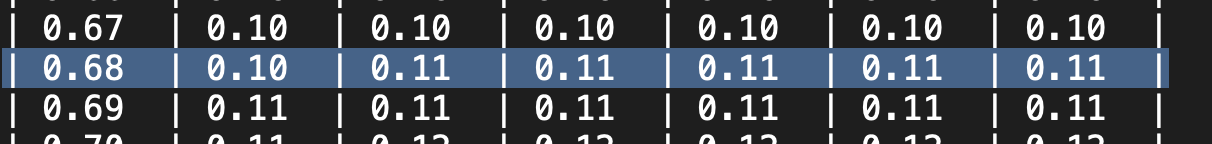
\includegraphics[scale = 0.6]{1.png}
	\caption{Интервал для первого приближения}
	\label{1approx}
\end{figure}

Интервал для второго приближения [-0.82; 0.82] (рис. \ref{2approx}).

\begin{figure}[h!p]
	\centering
	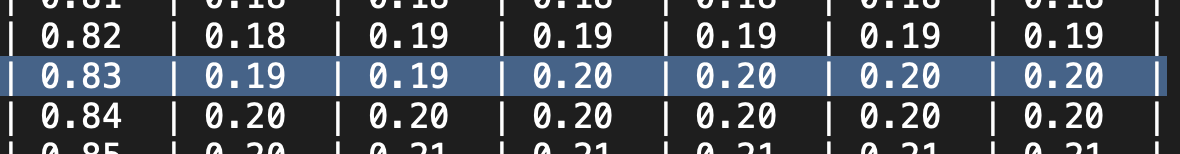
\includegraphics[scale = 0.6]{2.png}
	\caption{Интервал для второго приближения}
	\label{2approx}
\end{figure}

Интервал для третьего приближения [-1.27; 1.27] (рис. \ref{3approx}).

\begin{figure}[h!p]
	\centering
	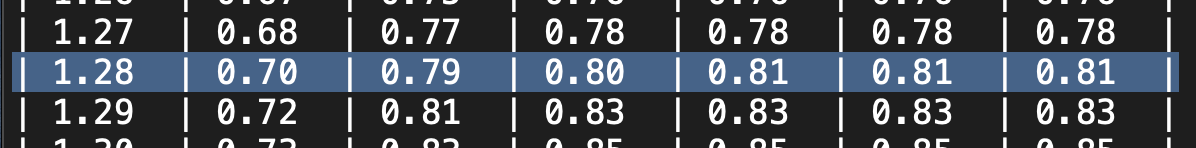
\includegraphics[scale = 0.6]{3.png}
	\caption{Интервал для третьего приближения}
	\label{3approx}
\end{figure}

Интервал для четвёртого приближения [-1.58; 1.58] (рис. \ref{4approx}).

\begin{figure}[h!p]
	\centering
	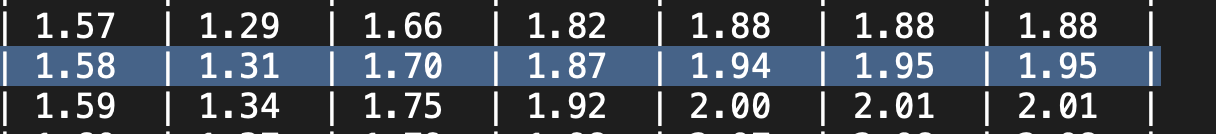
\includegraphics[scale = 0.6]{4.png}
	\caption{Интервал для четвертого приближения}
	\label{4approx}
\end{figure}
\newpage
\textbf{Вопрос 2.} Пояснить, каким образом можно доказать правильность полученного результата при фиксированном значении аргумента в численных методах.
	
\textbf{Ответ.} 

Доказать правильность полученного результата при фиксированном значении аргумента в численных методах можно с помощью уменьшения шага. Если при уменьшении шага полученный результат изменится незначительно, его можно считать правильным.

\textbf{Вопрос 3.}  Каково значение решения уравнения в точке x=2, т.е. привести значение u(2).
	
\textbf{Ответ.} 

При уменьшении шага (10e-2, 10e-3 .. 10e-7) видно, что значение u(2) стремится к 318 (рис. \ref{comp}). При этом анализируются значения, приведённые в 6 столбце (метод Рунге), так как он точнее метода Эйлера, а приближения Пикара при аргументе 2 нельзя считать решениями (показано в вопросе № 1). 

\begin{figure}[h!p]
	\centering
	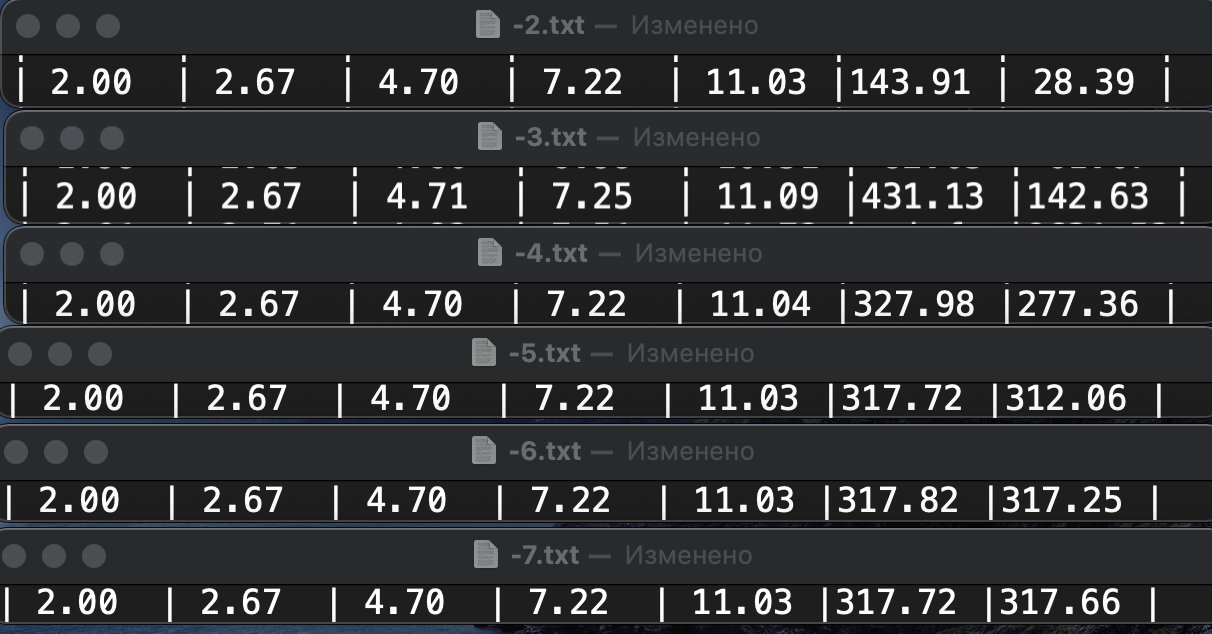
\includegraphics[scale = 0.6]{comp.png}
	\caption{Значение решения уравнения в точке x=2 при разном шаге}
	\label{comp}
\end{figure}
\textbf{Вопрос 4.}Дайте оценку точки разрыва решения уравнения.

\textbf{Ответ.} 
Точка разрыва второго рода в точке x = 2, так как решение уходит в бесконечность.
\newpage
\textbf{Вопрос 5.} Покажите, что метод Пикара сходится к точному аналитическому решению уравнения

\begin{displaymath}
u'(x) = x^ 2 + u,
\end{displaymath}
\begin{displaymath}
u(0) = 0
\end{displaymath}

\begin{figure}[h!p]
	\centering
	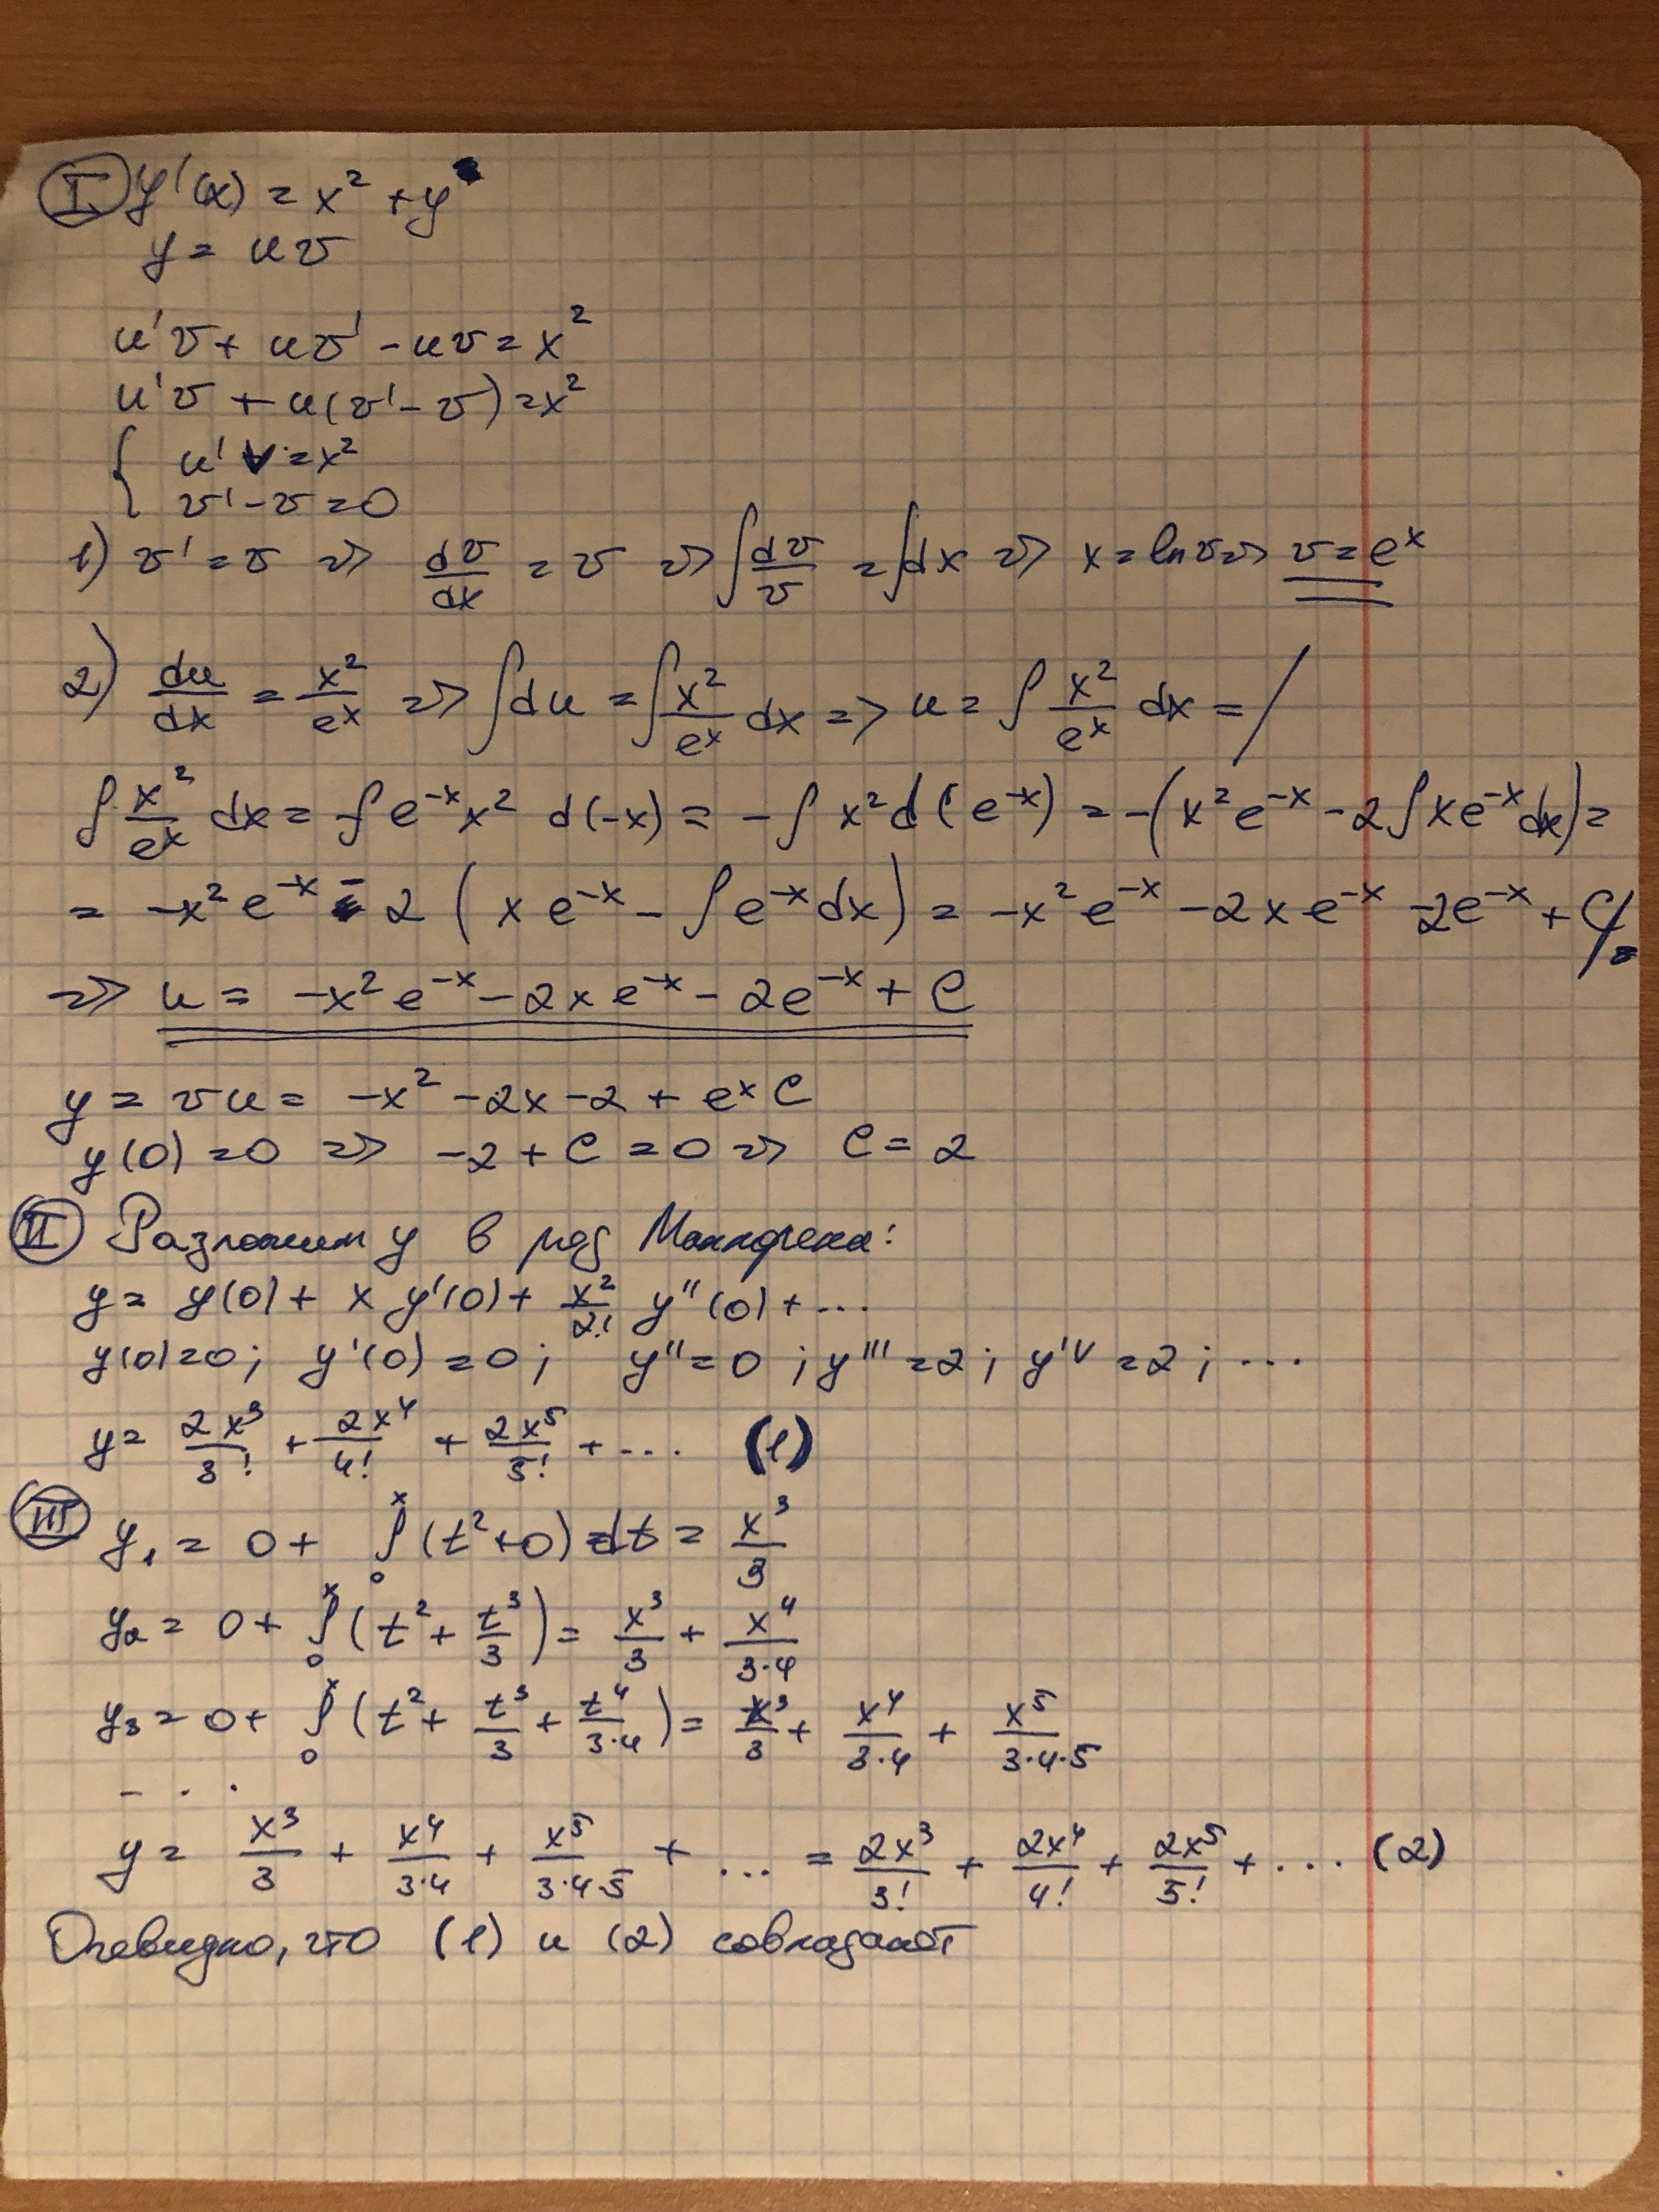
\includegraphics[scale=0.13]{solve.jpg}
	\caption{Решение}
	\label{comp}
\end{figure}

\end{document}